% Architecture diagram for README.md.
% Build: make diagram   (tectonic -> PDF -> pdftocairo -> SVG)
\documentclass[tikz,border=10pt]{standalone}
\usetikzlibrary{positioning,calc,arrows.meta,backgrounds,decorations.pathreplacing,fit}

\renewcommand{\familydefault}{\sfdefault}
\begin{document}
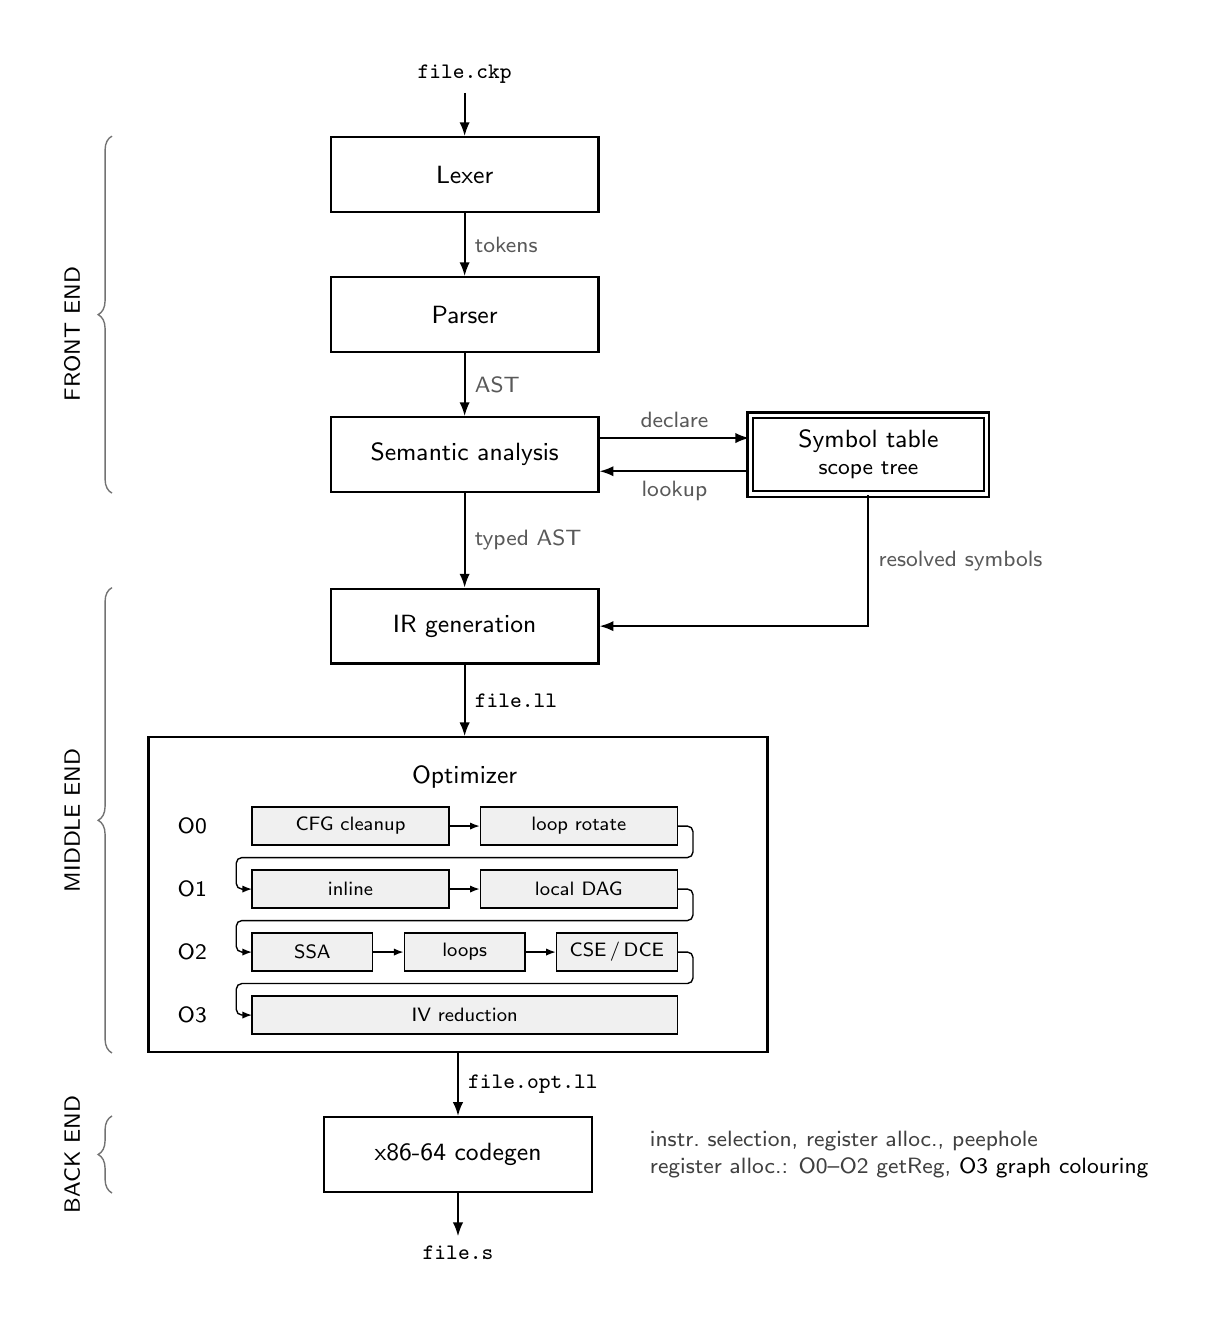
\begin{tikzpicture}[
    font=\small, node distance=0.8cm,
    stage/.style={draw, line width=0.8pt, minimum width=3.4cm, minimum height=0.95cm,
                  align=center, fill=white},
    store/.style={draw, line width=0.8pt, double, double distance=1.2pt,
                  minimum width=3cm, minimum height=1cm, align=center, fill=white},
    io/.style={font=\ttfamily\footnotesize},
    note/.style={font=\footnotesize, text=black!65, align=center},
    detail/.style={font=\footnotesize, align=left, text=black!75},
    arr/.style={-{Latex[length=5pt]}, line width=0.7pt},
    brace/.style={decorate, decoration={brace, amplitude=5pt, mirror}, line width=0.5pt, black!55},
    phase/.style={font=\footnotesize, text=black, rotate=90, anchor=south},
    pass/.style={draw, line width=0.5pt, fill=black!6, font=\scriptsize,
                 minimum height=0.48cm, inner xsep=2pt},
    lvl/.style={font=\footnotesize, anchor=east},
    passarr/.style={-{Latex[length=3.5pt]}, line width=0.5pt},
]

% main pipeline, top to bottom
\node[io] (src) {file.ckp};
\node[stage, below=0.55cm of src] (lex)   {Lexer};
\node[stage, below=of lex]        (parse) {Parser};
\node[stage, below=of parse]      (sema)  {Semantic analysis};
\node[stage, below=1.2cm of sema] (ir)    {IR generation};

% optimizer: one row per level, -On runs rows O0 to On in order.
% Every row is \rowW wide and centred on the pipeline; its passes share the width evenly.
\def\rowW{5.4}  \def\gap{0.4}
\path (ir.south) ++(0,-2.05) coordinate (r0);
\foreach \i/\t/\passes in {0/O0/{CFG cleanup,loop rotate},
                           1/O1/{inline,local DAG},
                           2/O2/{SSA,loops,CSE\,/\,DCE},
                           3/O3/{IV reduction}} {
  \path (r0) ++(0,-0.8*\i) coordinate (r\i);
  \node[lvl] (l\i) at ([xshift=-0.45cm]r\i -| -\rowW/2,0) {\t};
  \foreach \p [count=\k] in \passes { \xdef\n{\k} }
  \pgfmathsetmacro\w{(\rowW-(\n-1)*\gap)/\n}
  \foreach \p [count=\k from 0] in \passes {
    \node[pass, minimum width=\w cm] (p\i-\k) at ($(r\i)+({-\rowW/2+\w/2+\k*(\w+\gap)},0)$) {\p};
    \ifnum\k>0 \pgfmathtruncatemacro\prev{\k-1}\draw[passarr] (p\i-\prev) -- (p\i-\k); \fi
  }
  \coordinate (a\i) at ($(r\i)+(-\rowW/2,0)$);
  \coordinate (z\i) at ($(r\i)+(\rowW/2,0)$);
}
\foreach \i/\j in {0/1, 1/2, 2/3} {
  \coordinate (h\i) at ($(r\i)!0.5!(r\j)$);
  \draw[passarr, rounded corners=2pt] (z\i) -- ++(0.2,0) |- ([xshift=-0.2cm]h\i -| a\i) |- (a\j);
}
\node[anchor=south] (optT) at ([yshift=10pt]r0) {Optimizer};
\coordinate (mirror) at ([xshift=0.9cm]z3);
\node[draw, line width=0.8pt, inner sep=7pt, fit=(optT)(l3)(mirror)] (opt) {};

\node[stage, below=of opt]        (cg)    {x86-64 codegen};
\node[io, below=0.55cm of cg]     (asm)   {file.s};

\draw[arr] (src)   -- (lex);
\draw[arr] (lex)   -- node[note, right] {tokens} (parse);
\draw[arr] (parse) -- node[note, right] {AST}    (sema);
\draw[arr] (sema)  -- node[note, right] {typed AST} (ir);
\draw[arr] (ir)    -- node[io, right] {file.ll}     (ir |- opt.north);
\draw[arr] (opt.south -| cg) -- node[io, right] {file.opt.ll} (cg);
\draw[arr] (cg)    -- (asm);

% symbol table: built by semantic analysis, read by IR generation
\node[store, right=1.9cm of sema] (sym) {Symbol table\\[-1pt]{\footnotesize scope tree}};
\draw[arr] ([yshift=6pt]sema.east) -- node[note, above] {declare} ([yshift=6pt]sym.west);
\draw[arr] ([yshift=-6pt]sym.west) -- node[note, below] {lookup}  ([yshift=-6pt]sema.west -| sema.east);
\draw[arr] (sym.south) |- node[note, pos=0.25, right] {resolved symbols} (ir.east);

% codegen steps
\node[detail, anchor=west] at ([xshift=0.6cm]cg.east) {%
  instr.\ selection, register alloc., peephole\\
  register alloc.: O0--O2 getReg, {\color{black}O3 graph colouring}};

% phases
\coordinate (L) at ([xshift=-0.45cm]opt.west);
\draw[brace] (L |- lex.north) -- (L |- sema.south) node[midway, phase, xshift=-7pt, left=8pt, anchor=south] {FRONT END};
\draw[brace] (L |- ir.north)  -- (L |- opt.south)  node[midway, phase, left=8pt, anchor=south] {MIDDLE END};
\draw[brace] (L |- cg.north)  -- (L |- cg.south)   node[midway, phase, left=8pt, anchor=south] {BACK END};

\begin{scope}[on background layer]
  \fill[white] ([shift={(-10pt,-10pt)}]current bounding box.south west)
          rectangle ([shift={(10pt,10pt)}]current bounding box.north east);
\end{scope}
\end{tikzpicture}
\end{document}
